\chapter{Кинематика твердого тела. Вращательное движение вокруг неподвижной
оси.}

\begin{table}[h!]
    \vspace*{-2em}
    \begin{tabular}{C{.4}m{.55\textwidth}}
        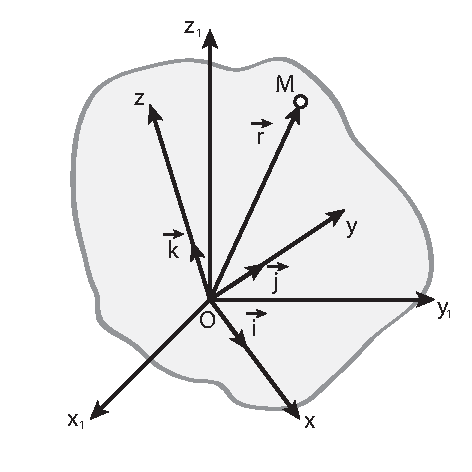
\includegraphics[width=.4\textwidth]{25_01} &
        Пусть твердое тело имеет одну неподвижную точку \( O \). Свяжем жестко
        с телом систему координат \( Oxyz \). Эта система координат однозначно
        определяет положение рассматриваемого тела по отношению к неподвижной
        системе отсчета \( Ox_1y_1z_1 \).

        Положение произвольной точки \( M \) твёрдого тела определяется
        радиус-вектором \( \vec{r} \). Пусть \( x,\ y,\ z \) -- это координаты
        точки \( M \) в подвижной системе, а \( \vec{i},\ \vec{j},\ \vec{k} \)
        -- орты этой системы координат. Тогда \( \vec{r} \):
        \( \vec{r} = x\vec{i} + y\vec{j} + z\vec{k} \).

        Координаты точки \( M \) в подвижной системе постоянны, а орты системы
        зависят от времени.
    \end{tabular}
    \vspace*{-1.5em}
\end{table}

Тогда скорость точки \( M \) равна: \( \ds \vec{v} = \der{\vec{r}}{t} =
x\der{\vec{i}}{t} + y\der{\vec{j}}{t} + z\der{\vec{k}}{t} \).

Умножая обе части равенства скалярно на орты \( \vec{i},\ \vec{j},\ \vec{k} \),
получим:
\[
    \left\{ \begin{array}{l}
        \ds v_x = \vec{v}\cdot\vec{i} = x\der{\vec{i}}{t}\cdot\vec{i} +
        y\der{\vec{j}}{t}\cdot\vec{i} + z\der{\vec{k}}{t}\cdot\vec{i}, \\[.4em]
        \ds v_y = \vec{v}\cdot\vec{j} = x\der{\vec{i}}{t}\cdot\vec{j} +
        y\der{\vec{j}}{t}\cdot\vec{j} + z\der{\vec{k}}{t}\cdot\vec{j}, \\[.4em]
        \ds v_z = \vec{v}\cdot\vec{k} = x\der{\vec{i}}{t}\cdot\vec{k} +
        y\der{\vec{j}}{t}\cdot\vec{k} + z\der{\vec{k}}{t}\cdot\vec{k}.
    \end{array} \right.
\]

Так векторы \( \vec{i},\ \vec{j},\ \vec{k} \) взаимно перпендикулярны, то
\[
    \vec{i}^2 = 1,\ \vec{j}^2 = 1,\ \vec{k}^2 = 1, \quad
    \vec{i}\cdot\vec{j} = 0,\ \vec{j}\cdot\vec{k} = 0,\ \vec{k}\cdot\vec{i} = 0.
\]

Дифференцируя по времени, получим:
\[
    \der{\vec{i}}{t}\cdot\vec{i} = 0,\ \der{\vec{j}}{t}\cdot\vec{j} = 0,\ 
    \der{\vec{k}}{t}\cdot\vec{k} = 0, \quad 
    \der{\vec{i}}{t}\cdot\vec{j} = -\der{\vec{j}}{t}\cdot\vec{i},\ 
    \der{\vec{j}}{t}\cdot\vec{k} = -\der{\vec{k}}{t}\cdot\vec{j},\ 
    \der{\vec{k}}{t}\cdot\vec{i} = -\der{\vec{i}}{t}\cdot\vec{k}.
\]

Тогда система принимает вид:
\[
    \left\{ \begin{array}{l}
        \ds v_x = z\der{\vec{k}}{t}\cdot\vec{i} - y\der{\vec{i}}{t}\cdot\vec{k},
        \\[.4em]
        \ds v_y = x\der{\vec{i}}{t}\cdot\vec{j} - z\der{\vec{j}}{t}\cdot\vec{i},
        \\[.4em]
        \ds v_z = y\der{\vec{j}}{t}\cdot\vec{k} - x\der{\vec{k}}{t}\cdot\vec{j}.
    \end{array} \right.
\]
Эти формулы содержат три скалярные функции, которые обозначим как:
\[
    \omega_x = \der{\vec{j}}{t}\cdot\vec{k},\ \omega_y =
    \der{\vec{k}}{t}\cdot\vec{i},\ \omega_z = \der{\vec{i}}{t}\cdot\vec{j}.
\]

Тогда система примет вид \( v_x = z\omega_y - y\omega_z,\ v_y = x\omega_z -
z\omega_x,\ v_z = y\omega_x - x\omega_y \), а скорость: \( \vec{v} =
(z\omega_y - y\omega_z)\vec{i} + (x\omega_z - z\omega_x)\vec{j} +
(y\omega_x - x\omega_y)\vec{k} \).

Введем вектор \( \vec{\omega} = \{\omega_x, \omega_y, \omega_z\} \), тогда можно
представить скорость точки в виде векторного произведения:
\( \vec{v} = \vec{\omega}\times\vec{r} \).

Найдем ускорение произвольной точки твердого тела. Введем понятие углового
ускорения: производная угловой скорости по времени, то есть
\( \ds \vec{\eps} = \der{\vec{\omega}}{t} \).

Найдем ускорение точки \( M \):
\[
    \vec{a} = \der{\vec{v}}{t} = \der{(\vec{\omega}\times\vec{r})}{t} =
    \der{\vec{\omega}}{t}\times\vec{r} + \vec{\omega}\times\der{\vec{r}}{t} =
    \vec{\eps}\times\vec{r} + \vec{\omega}\times\vec{v}.
\]
Таким образом, ускорение может быть представлено как сумма двух ускорений:
первое слагаемое называется вращательной составляющей ускорения, а второе --
осестремительной.

\newpage
